        \title[\whatshort, \simplenum, 
Slide \insertframenumber/\inserttotalframenumber ] {\what}
% this dirty hack allows me to display frame numbers in the footnotebar.

 

\subtitle{Class \simplenum: Reinforcement Learning}



\usepackage{graphicx}
%\subtitle{}

\begin{document}

\begin{frame}
  \titlepage

\end{frame}

\begin{frame}
  \frametitle{Class Outline} \tableofcontents % You might wish to add
  %the option [pausesections]
\end{frame}


% Since this a solution template for a generic talk, very little can
% be said about how it should be structured. However, the talk length
% of between 15min and 45min and the theme suggest that you stick to
% the following rules:  

% - Exactly two or three sections (other than the summary).
% - At *most* three subsections per section.
% - Talk about 30s to 2min per frame. So there should be between about
%   15 and 30 frames, all told.

\begin{frame}[fragile]
\frametitle{References}

\begin{itemize}

\item[[TM{]}] T.~M.~Mitchell, ``Machine Learning'', McGraw-Hill, 1998,
  Chapter 13.

\item[[SB{]}] R.~S.~Sutton and A.~G.~Barto, 
``Reinforcement Learning: An Introduction'', 2nd edition, The MIT
Press, 2018

\item[[CS{]}]  C.~Szepesv\'ari
``Algorithms for Reinforcement Learning'', Morgan \& Claypool, 2010

\item[[JT{]}] J.~N.~Tsitsiklis, On the Convergence of Optimistic Policy
Iteration, JMLR 3 (2002) 59-72

\item[[WD{]}] C.~J.~C.~H.~Watkins and P.~Dayan, Technical Note:
Q-Learning, Machine Learning, 8, 279-292 (1992)

\end{itemize}
\end{frame}

\section[Preliminaries]{Motivation and Preliminaries}

\begin{frame}\frametitle{Principal Setup}

\begin{itemize}

\item a learning agent interacts with an environment

--- the agent takes an action

--- the environment gives a reward and changes its state

\bigskip

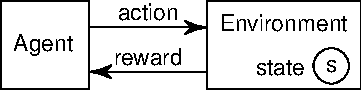
\includegraphics[scale=1]{agent_environment}

\item we make the Markov assumption: all activity (choice of the
action, reward, state to go to) depends on the
current state rather then the whole history

--- given the current state, the future is independent of the past

\item the current state is visible to the agent

\end{itemize}
\end{frame}


\begin{frame}\frametitle{Gridworlds}
\begin{itemize}

\item gridworlds are toy examples used to illustrate principles of
reinforcement learning

\bigskip

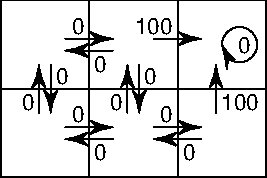
\includegraphics[scale=1]{gridworld}
\begin{minipage}{5cm}
~~~~~~~~~~~~(after [TM], Fig.~13.2)
\end{minipage}

\item the agent can move from a square to a neighbouring square; the
rewards are shown on the diagram

\item here the top right corner is a \alert{goal state (or terminal
state)}; further moves from it are neither possible nor needed

\end{itemize}
\end{frame}

\begin{frame}\frametitle{Deterministic Environment}
\begin{itemize}

\item this example is a deterministic environment

--- the reward and the state we move into are functions of the current
    state and action taken

\item let $S$ be the set of all states and $A$ be the set of all
    actions; if the environment is deterministic, then


--- reward $r = \text{Reward}(s,a)$, where $\text{Reward}: S\times
    A\to R$ is a function

--- state we move into $s = \text{State}(s,a)$, where $\text{State}:
    S\times A$ is a function

\item the environment can be described by two functions

\end{itemize}
\end{frame}

\begin{frame}\frametitle{Stochastic Environment}
\begin{itemize}

\item suppose we are controlling a robot in a real-life situation

\item there is uncertainty as to what happens after an action

--- the reward we get and the state we move into after taking an
    action $a$ in a state $s$ can be modelled by random variables
    $\text{Reward}_{s,a}$ and $\text{State}_{s,a}$

\item the environment may be described by a collection of
    distributions on $R\times S$

--- there is one distribution for each pair $(s,a)$

\item this is called a \alert{Markov Decision Process (MDP)}

\item we assume the MDP is stationary, i.e., if we return to state $s$
and choose the same action $a$, we are faced with the same possibilities

\end{itemize}
\end{frame}

\end{document}










